\documentclass[10pt]{scrartcl}

\usepackage[utf8]{inputenc}
\usepackage{tabularx}
\usepackage{longtable}
\usepackage[ngerman]{babel}
\usepackage[automark]{scrpage2}
\usepackage{amsmath,amssymb,amstext}
%\usepackage{mathtools}
\usepackage[]{color}
\usepackage[]{enumerate}
\usepackage{graphicx}
\usepackage{lastpage}
\usepackage[perpage,para,symbol*]{footmisc}
\usepackage{listings} 
\usepackage[pdfborder={0 0 0},colorlinks=false]{hyperref}
\usepackage[numbers,square]{natbib}
\usepackage{color}
\usepackage{colortbl}
\usepackage[absolute]{textpos}
\usepackage{float}
\usepackage[colorinlistoftodos,textsize=small,textwidth=2cm,shadow,bordercolor=black,backgroundcolor={red!100!green!33},linecolor=black]{todonotes}

\lstset{numbers=left, numberstyle=\tiny, numbersep=5pt, breaklines=true, showstringspaces=false} 
\restylefloat{figure}

%changehere
\def\titletext{Praktikum 1 : Stellen/Transitionsnetze}
\def\titletextshort{Praktikum 1}
\author{André Harms, Oliver Steenbuck}

\title{\titletext}

%changehere Datum der Übung
\date{04.04.2012}

\pagestyle{scrheadings}
%changehere
\ihead{TH1, Padberg}
\ifoot{Generiert am:\\ \today}


\cfoot{Oliver Steenbuck, André Harms}


\ohead[]{\titletextshort}
\ofoot[]{{\thepage} / \pageref{LastPage}}

\setlength{\parindent}{0.0in}
\setlength{\parskip}{0.1in}

\begin{document}
\maketitle

\setcounter{tocdepth}{3}
\tableofcontents

%	\listoftables                                 												% 
	\listoffigures  
%	\lstlistoflistings	

\section{Aufgabe 1}
	\begin{figure}[H]
        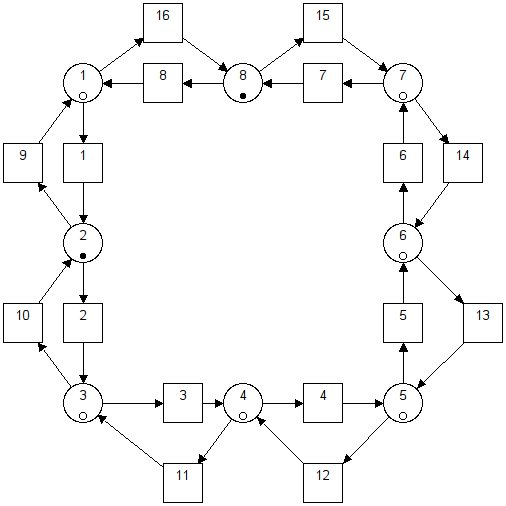
\includegraphics[width=\textwidth]{aufgabe1.png}
        \caption{Simples Gleis}
        \label{img:aufg1}
	\end{figure}
	
	Hier repräsentiert jeder Token einen Zug, der jeweils in beide Richtungen von Gleisabschnitt (Stelle) zu Gleisabschnitt (Stelle) fahren können, sofern in dem betreffenden Abschnitt noch kein Zug vorhanden ist. Die Eigenschaft eines Zuges exklusiv einen Gleisabschnitt zu besetzen, haben wir über Kapazitäten der Stellen modelliert.
	
\section{Aufgabe 2}
	\subsection{Schranke}	
		\begin{figure}[H]
			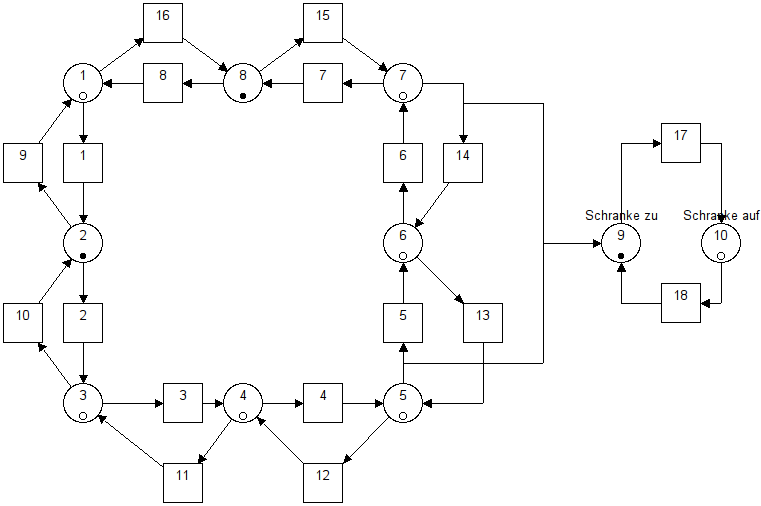
\includegraphics[width=\textwidth]{aufgabe21.png}
        	\caption{Schranke}
        	\label{img:aufg2}
		\end{figure}
	Durch die Schranke wird der Zugang zum Gleisabschnitt 6 kontrolliert. Bei geschlossener Schranke kann ein Zug in diesen einfahren, bei geöffneter Schranke nicht. Die Schranke kann geöffnet werden während sich ein Zug im Gleisabschnitt 6 befindet\footnote{Es ergibt sich für Fußgänger und Autofahrer die Chance einen Darwin Award zu erhalten}.

\subsection{Weiche}	
	\begin{figure}[H]
		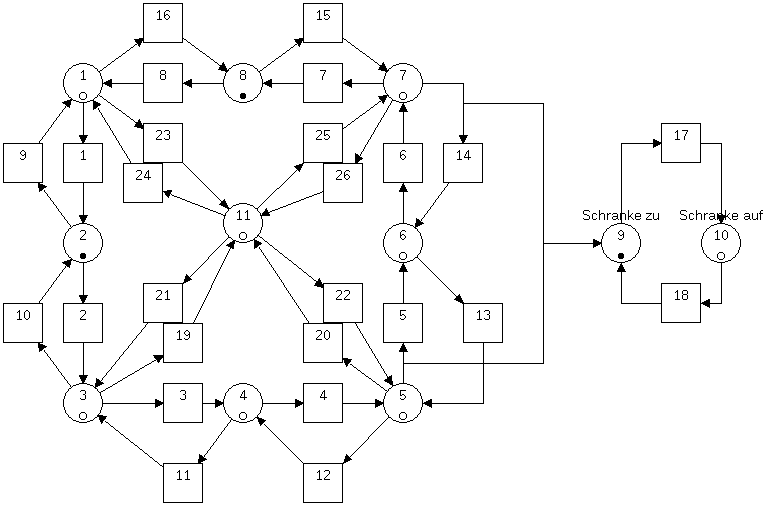
\includegraphics[width=\textwidth]{aufgabe22.png}
       	\caption{Weiche}
       	\label{img:aufg2}
	\end{figure}


Die Weiche - die die Form einer 8 ermöglicht - wird durch eine Stelle in der Mitte der Eckstellen repräsentiert. Züge können somit eine 8 oder aber auch \glqq{}im Zickzack\grqq (1-11-7) fahren.

\section{Weiche}
		
		\subsection{S Invarianten}
	
			
\begin{table}[H]
\centering		
		\begin{tabular}{|c|c|c|}
\hline Stelle  & $W_1$ & $W_2$ \\ 
\hline S1 & 0 & 1 \\ 
\hline S2 & 0 & 1 \\ 
\hline S3 & 0 & 1 \\ 
\hline S4 & 0 & 1 \\ 
\hline S5 & 0 & 1 \\ 
\hline S6 & 0 & 1 \\ 
\hline S7 & 0 & 1 \\ 
\hline S8 & 0 & 1 \\ 
\hline S9 & 1 & 0 \\ 
\hline S10 & 1  & 0 \\ 
\hline S11 & 0 & 1 \\
\hline 
\end{tabular}
\caption{S Invarianten}
\end{table}
Wir suchen zwei Invarianten. Eine die zeigt, dass kein Zug verschwindet und keiner hinzukommt und eine die zeigt, daß die Schranke funktioniert. 
Wir sehen in Spalte $W_1$, dass die Stellen S9 und S10 die die Schranke darstellen im Gleichgewicht sind und jeweils immer nur eine der Positionen \verb!Schranke auf! bzw. \verb!Schranke zu! haben kann.  
In Spalte $W_2$ sehen wir, dass die Anzahl der Züge immer gleichbleibt (wenn wir $M_0$ mitbetrachten sehen wir das es immer 2 Züge sind). 

\subsection{T Invarianten}
	\subsubsection{Wiederhohltes Schalten der Schranke}
	Wir erwarten, das wenn die Schrankentransistionen $T_{17}$ $T_{18}$ beliebig oft aber immer beide geschaltet werden die Schranke wieder im Ursprungszustand ist. Dies können wir in der in Tabelle \ref{t:inv:schrank} gezeigten Invariante sehen. 
	\begin{table}[H]
	\centering	
		\begin{tabular}{|c|c|}
	\hline Trans.  & $W_1$\\ 
	\hline $T_{1-16}$ & 0  \\ 
	\hline $T_{17}$ & 1 \\ 
	\hline $T_{18}$ & 1 \\ 
	\hline $T_{19-26}$ & 0 \\ 
	\hline 
	\end{tabular}
	\caption{T Invarianten}
	\label{t:inv:schrank}
	\end{table}	
	
\subsubsection{Vor und zurückfahren}
	Da jeder Gleisabschnitt in beide Richtungen befahrbar ist erwarten wir, dass es T-Invarianten bei für einen Zug gibt der immer zwischen denselben beiden Gleisabschnitten hin- und herfährt. Tabelle \ref{t:inv:vorzurueck} Zeigt diese Invariante für die Transitionen $T_1$ und $T_9$ die die Stellen $S_1$ und $S_2$ in beide Richtungen verbinden. 
	\begin{table}[H]
	\centering	
		\begin{tabular}{|c|c|}
	\hline Trans.  & $W_1$\\ 
	\hline $T_{1}$ & 1 \\
	\hline $T_{2-8}$ & 0  \\ 
	\hline $T_{9}$ & 1 \\ 
	\hline $T_{10-26}$ & 0 \\ 
	\hline 
	\end{tabular}
	\caption{T Invarianten}
	\label{t:inv:vorzurueck}
	\end{table}	
	
\subsection{Erreichbarkeitsgraph}
Im Erreichbarkeitsgraph sehen wir keine Auffälligkeiten. Es sind immer genau 3 Token vorhanden von dennen sich eines in der Schranke ($T_{17}$, $T_{18}$) befindet und 2 andere auf Gleisabschnitten.

\subsection{Überdeckungsgraph}
Der Überdeckungsgraph ist für Stellen mit Kapazitäten hier gleich dem Erreichbarkeitsgraphen und wird daher nicht näher betrachtet.\\
Es zeigen sich auch keine weiteren Auffälligkeiten wie z.B. Senken die auf Deadlocks hindeuten würden. Insofern erfüllen sich die Erwartungen die bei uns nach der Netzkonstruktion entstanden sind. Es handelt sich um eine Lebendiges Netz in dem es keine Deadlocks gibt und das im wesentlichen aus 2 Kreisläufen (Züge und Schranke) besteht.

\subsection{Kondensationsgraph}
Der Kondensationsgraph zeigt nur einen Knoten, da bei der von uns gewählten Modellierung alle Knoten eine starke Verbindung aufweisen. Wir schließen daraus, dass ein Zug alle Schienenabschnitte erreichen kann. 

\subsection{Mehr Züge}	
An den oben gezeigten Korrektheitseigenschaften ändert sich nichts. Die Graphen werden komplexer da mit mehr Token noch mehr Möglichkeiten bestehen. Erwartungsgemäß nehmen die Möglichkeiten verschieden Transitionen zu schalten bei bis zu 4 Zügen zu um dann ab 6 Zügen wieder abzunehmen bis bei 9 Zügen nur noch die Schranke gestellt werden werden kann da die Züge sich gegenseitig blockieren.

		
\end{document}

